\chapter{自旋与两能级系统}\label{ch:b3:spin-two-level}

1922 年，斯特恩和盖拉赫让一束银原子穿过一个非均匀磁铁，
原以为原子要么不偏转，要么形成连续的涂抹状分布。
束流却干净利落地分裂为\emph{两}束。轨道角动量
无法做到这一点：$2l + 1$ 永远是奇数。原子
宣告了一种全新的、纯粹量子的属性——\emph{\omterm{def:b3:spin-two-level:spin}{自旋}}，它是一种
内禀角动量，$j = \tfrac12$，是半整数阶梯，
在\cref{ch:b3:quantum-angular-momentum}中代数预留的，
轨道运动永远用不上。\omterm{def:b3:spin-two-level:spin}{自旋}使每个电子态加倍（完成了
周期表背后的计数），承载着铁的磁性，
以及质子的磁性，并且是自然界所提供的最纯粹的
两能级系统。本章的物理支撑着
每家医院里的\omterm{prop:b3:spin-two-level:rabi}{磁共振}扫描仪、定义秒的铯原子钟、
用于测绘星系的 21 厘米射电辐射，以及量子比特。

\section{发现自旋的实验}

\begin{example}[斯特恩–盖拉赫实验]\label{ex:b3:spin-two-level:stern-gerlach}
磁矩 $\vect\mu$ 处于\emph{非均匀}磁场中时受到的力为
$F_z = \mu_z\,\partial B_z/\partial z$：偏转量
即测得 $\mu_z$。经典预期：磁矩随机取向，
形成连续的扇形分布。轨道角动量的量子预期：$2l + 1$
个斑点：一个、三个、五个——总是奇数。实际观测（银
原子，氢原子同样）：\emph{两}个对称斑点，中间没有任何分布。
被测分量恰好取两个值——这正是 $j
= \tfrac12$ 的特征，轨道运动不允许，也是量子化的直接展示：
仪器本质上是测量单一\omterm{def:b3:spin-two-level:spin}{自旋}分量的装置，
束流分裂为其两个\omterm{def:b3:quantum-formalism:observable}{本征值}。
\end{example}

\begin{omfigure}
\begin{tikzpicture}[font=\small, >=Stealth]
  % oven
  \fill[omExo!25, draw=omExo] (0,-0.4) rectangle (1.1,0.4);
  \node[font=\footnotesize] at (0.55,-0.75) {炉};
  \draw[->, thick] (1.2,0) -- (2.6,0);
  % magnet
  \fill[omDef!20, draw=omDef, thick] (2.8,0.35) -- (4.8,0.35) -- (4.8,1.15) -- (2.8,1.15) -- cycle;
  \draw[omDef, thick] (3.3,0.35) -- (3.8,0.75) -- (4.3,0.35);
  \fill[omDef!20, draw=omDef, thick] (2.8,-0.35) rectangle (4.8,-1.05);
  \node[omDef, font=\footnotesize] at (3.8,1.45) {N（尖端）};
  \node[omDef, font=\footnotesize] at (3.8,-1.35) {S};
  % beams
  \draw[omThm, very thick] (2.6,0) -- (4.8,0.1) -- (7.2,0.85);
  \draw[omThm, very thick] (2.6,0) -- (4.8,-0.1) -- (7.2,-0.85);
  % screen
  \draw[thick] (7.4,-1.5) -- (7.4,1.5);
  \fill[omThm] (7.4,0.85) circle (2.6pt);
  \fill[omThm] (7.4,-0.85) circle (2.6pt);
  \node[anchor=west, font=\footnotesize] at (7.6,0.85) {$S_z = +\hbar/2$};
  \node[anchor=west, font=\footnotesize] at (7.6,-0.85) {$S_z = -\hbar/2$};
  \node[anchor=west, font=\footnotesize, gray] at (7.6,0) {（经典涂抹：不存在）};
\end{tikzpicture}

{\small 斯特恩–盖拉赫实验：非均匀磁场将
方向相反的磁矩拉向相反的方向，使磁铁成为测量单一\omterm{def:b3:spin-two-level:spin}{自旋}分量的
仪器。银原子落在两个斑点上——一个两值可观测量，
正被当场捕获。}
\end{omfigure}

\begin{definition}[自旋一半]\label{def:b3:spin-two-level:spin}
\index{自旋}\index{泡利矩阵}\index{旋量}
电子（以及质子、中子、夸克）带有
内禀角动量，$j = \tfrac12$：其态空间为二维
由 $\ket\uparrow, \ket\downarrow$ 张成（它们是
$\hat S_z$ 的本征态，\omterm{def:b3:quantum-formalism:observable}{本征值}为 $\pm\hbar/2$）。在此空间上
\[
\hat{\vect S} = \frac\hbar2\,\hat{\vect\sigma} , \qquad
\sigma_x = \begin{pmatrix}0&1\\1&0\end{pmatrix} ,\;
\sigma_y = \begin{pmatrix}0&-\iu\\\iu&0\end{pmatrix} ,\;
\sigma_z = \begin{pmatrix}1&0\\0&-1\end{pmatrix}
\]
——即\emph{泡利矩阵}，它以最小可能的空间
实现了角动量代数。一般态
$\alpha\ket\uparrow + \beta\ket\downarrow$ 称为\emph{旋量}。电子的
磁矩为
\[
\hat{\vect\mu} = -g\,\frac{\mu_{\text{B}}}{\hbar}\,\hat{\vect S} ,
\qquad g \approx 2 :
\]
即单位角动量对应的磁矩是轨道情形的两倍——这一反常现象
是爱因斯坦–德哈斯实验曾测得的
（见\cref{exo:b3:quantum-angular-momentum:12}），狄拉克方程
后来也给出了这一结果。自旋并非任何物体的转动：没有半径，
也没有“自旋的小球”能经得起推敲——它是内禀的，像
正如电荷。
\end{definition}

\begin{example}[级联斯特恩–盖拉赫滤波器]\label{ex:b3:spin-two-level:chained}
选取 $S_z = +\hbar/2$ 的束流，再次测量 $S_z$：全部
原子的结果都是 $+$。改测 $S_x$：各占一半——态
$\ket\uparrow$ 是 $(\ket{+x} + \ket{-x})/\sqrt2$ 的叠加。
现在保留 $S_x = +$ 的束流，再测一次 $S_z$：
各占一半\emph{再次}出现——$S_x$ 的测量抹去了先前
尖锐的 $S_z$。三个磁铁足以展示不相容性、
坍缩与玻恩定则；这一链条正是
用原子完成的\cref{ex:b3:quantum-formalism:threepolarizers}。
\end{example}

\section{布洛赫球}

\begin{proposition}[沿任意轴的自旋]\label{prop:b3:spin-two-level:bloch}
\index{布洛赫球}
对单位方向 $\vect n = (\sin\theta\cos\varphi,
\sin\theta\sin\varphi, \cos\theta)$，算符 $\vect
n\cdot\hat{\vect\sigma}$ 的\omterm{def:b3:quantum-formalism:observable}{本征值}为 $\pm1$，且
\[
\ket{+\vect n} = \cos\tfrac\theta2\,\ket\uparrow +
\eu^{\iu\varphi}\sin\tfrac\theta2\,\ket\downarrow .
\]
每个纯\omterm{def:b3:spin-two-level:spin}{旋量}恰好为某一个方向的 $\ket{+\vect n}$，且该方向唯一：态空间
映射到一个球面上——\emph{\omterm{prop:b3:spin-two-level:bloch}{布洛赫球}}——
正交态位于\emph{对跖点}上（注意半角：相反方向
而非垂直方向才是正交的）。球面上的旋转
恰好就是磁场所产生的演化：
这是迄今为止每一次量子比特操控的几何基础。
\end{proposition}

\begin{proof}[部分证明]
对角化 $2\times2$ 矩阵 $\vect n\cdot\vect\sigma =
\begin{pmatrix}\cos\theta & \sin\theta\,\eu^{-\iu\varphi}\\
\sin\theta\,\eu^{\iu\varphi} & -\cos\theta\end{pmatrix}$：迹为 $0$，
行列式为 $-1$，\omterm{def:b3:quantum-formalism:observable}{本征值}为 $\pm1$；给定的\omterm{def:b3:spin-two-level:spin}{旋量}可通过
代入验证（利用半角公式）。对跖点：$\theta \to \pi -
\theta$，$\varphi \to \varphi + \pi$，则有 $\braket{+\vect
n'}{+\vect n} = 0$。
\end{proof}

\begin{omfigure}
\begin{tikzpicture}[font=\small, >=Stealth]
  \draw[gray!70] (0,0) circle (2.1);
  \draw[gray!70, dashed] (0,0) ellipse (2.1 and 0.6);
  \draw[->] (0,0) -- (0,2.75);
  \node[anchor=south] at (0,2.75) {$z$: $\ket\uparrow$};
  \node[anchor=north, font=\footnotesize] at (0,-2.2) {$\ket\downarrow$};
  \draw[->] (0,0) -- (2.7,-0.55);
  \node[anchor=west] at (2.7,-0.55) {$x$};
  \draw[->] (0,0) -- (1.35,0.62);
  \node[anchor=west] at (1.35,0.66) {$y$};
  % state vector
  \draw[->, omDef, very thick] (0,0) -- (55:2.1);
  \node[omDef, anchor=south west] at (55:2.1) {$\ket{+\vect n}$};
  \draw[omDef, dashed] (0,1.1) arc (90:55:1.1);
  \node[omDef, font=\footnotesize] at (72:1.42) {$\theta$};
  % equator states
  \fill[omThm] (2.1,0) circle (2pt);
  \node[omThm, anchor=west, font=\footnotesize] at (2.2,0.12)
    {$(\ket\uparrow + \ket\downarrow)/\sqrt2$};
\end{tikzpicture}

{\small \omterm{prop:b3:spin-two-level:bloch}{布洛赫球}：每个自旋-$\tfrac12$ 态对应球面上的一点；
两极为 $\ket\uparrow, \ket\downarrow$，赤道上是它们的
等幅叠加，正交态位于对跖点上。
磁场使球面旋转——这是量子比特的
“控制面板”。}
\end{omfigure}

\section{磁场中的自旋：进动与共振}

\begin{proposition}[拉莫尔进动]\label{prop:b3:spin-two-level:larmor}
\index{拉莫尔进动}\index{旋磁比}
在静磁场 $\vect B_0 = B_0\vect e_z$ 中，\omterm{def:b3:hamiltonian-mechanics:hamiltonian}{哈密顿量} $\hat
H = -\hat{\vect\mu}\cdot\vect B_0$ 将两能级分裂为
$\hbar\omega_0$，并使平均\omterm{def:b3:spin-two-level:spin}{自旋}
绕磁场\emph{进动}：
\[
\frac{\dd\langle\hat{\vect S}\rangle}{\dd t} =
\gamma\,\langle\hat{\vect S}\rangle\wedge\vect B_0 , \qquad
\omega_0 = |\gamma|B_0 ,
\]
其中\omterm{prop:b3:spin-two-level:larmor}{旋磁比}为 $\gamma$（$\mu = \gamma S$）。布洛赫
矢量绕 $z$ 轴以 $\omega_0$ 转动，其与磁场的夹角保持不变
——正是经典陀螺的图像，在此处严格成立，因为
\omterm{def:b3:quantum-formalism:commutator}{对易子}是线性的。对电子：$\qty{28}{GHz/T}$；对
质子（磁矩为 $2.79$ 核磁子）：$\gamma_p/2\pi =
\qty{42.6}{MHz/T}$——每台核\omterm{prop:b3:spin-two-level:rabi}{磁共振}成像仪的“车牌号”。
\end{proposition}

\begin{proof}
应用\cref{prop:b3:quantum-formalism:evolution}，取 $\hat H =
-\gamma B_0\hat S_z$：\omterm{def:b3:quantum-formalism:commutator}{对易子}给出 $\dd\langle\hat
S_x\rangle/\dd t = -\gamma B_0\langle\hat S_y\rangle$，
$\dd\langle\hat S_y\rangle/\dd t = +\gamma B_0\langle\hat
S_x\rangle$，$\dd\langle\hat S_z\rangle/\dd t = 0$，三者
合成为所述的矢量积。
\end{proof}

\begin{proposition}[磁共振]\label{prop:b3:spin-two-level:rabi}
\index{磁共振}\index{拉比振荡}
加上一个在横向平面内转动的弱磁场 $B_1$，
其频率为 $\omega$。在随之转动的参考系中，$B_0$ 有效地
降为 $(\omega_0 - \omega)/|\gamma|$；\emph{共振
时}（$\omega = \omega_0$）下仅 $B_1$ 起作用，\omterm{def:b3:spin-two-level:spin}{自旋}绕它
进动，以\emph{拉比频率} $\Omega_1 =
|\gamma|B_1$：从 $\ket\uparrow$ 出发，翻转
的概率为
\[
\mathcal P_\downarrow(t) = \sin^2\Big(\frac{\Omega_1t}{2}\Big) .
\]
持续时间为 $\pi/\Omega_1$ 的脉冲（“$\pi$ 脉冲”）使\omterm{def:b3:spin-two-level:spin}{自旋}
反转；其一半（“$\pi/2$ 脉冲”）使其
位于赤道面内，此时\omterm{def:b3:spin-two-level:spin}{自旋}以 $\omega_0$ 进动，并通过法拉第电磁感应，
将其频率\emph{广播}到附近任一线圈中。偏离共振时，
翻转振幅按 $\Omega_1^2/[\Omega_1^2 +
(\omega - \omega_0)^2]$ 急剧衰减：响应具有强烈的选择性，
即共振——这正是使\omterm{def:b3:spin-two-level:spin}{自旋}能够被
逐种、并借助场梯度逐点寻址的原因
（见\cref{pb:b3:spin-two-level:1}）。
\end{proposition}
\admitted

\begin{omfigure}
\begin{tikzpicture}
  \begin{axis}[omaxis, axis x line=bottom, axis y line=left,
    width=7.0cm, height=4.8cm, xmin=0, xmax=3, ymin=0, ymax=1.15,
    xlabel={$t$（单位 $2\pi/\Omega_1$）}, ylabel={$\mathcal P_\downarrow$},
    xlabel style={at={(axis description cs:0.5,-0.12)}, anchor=north},
    xtick={0.5,1,1.5,2,2.5}, ytick={0.5,1}, clip=false]
    \addplot[omDef, very thick, domain=0:3, samples=160]
      {sin(deg(pi*x))^2};
    \addplot[omExo, thick, dashed, domain=0:3, samples=160]
      {0.36*sin(deg(pi*x/0.6))^2};
    \node[omDef, font=\scriptsize, anchor=south] at (axis cs:0.5,1.01) {共振};
    \node[omExo, font=\scriptsize, anchor=west] at (axis cs:1.72,0.52) {失谐};
  \end{axis}
  \begin{scope}[xshift=8.9cm, yshift=0.4cm, >=Stealth]
    \draw[->, thick] (0,-0.3) -- (0,3.1);
    \node[anchor=south] at (0,3.1) {$\vect B_0$};
    \draw[gray, dashed] (0,1.9) ellipse (1.15 and 0.34);
    \draw[->, omDef, very thick] (0,0) -- (1.05,2.05);
    \draw[->, omDef] (1.18,2.06) arc (5:130:1.16 and 0.35);
    \node[omDef, font=\footnotesize, anchor=west] at (1.15,1.35) {$\langle\vect S\rangle$};
    \node[font=\footnotesize, anchor=west] at (0.75,2.85) {$\omega_0 = |\gamma|B_0$};
  \end{scope}
\end{tikzpicture}

{\small 左图：\omterm{prop:b3:spin-two-level:rabi}{拉比振荡}——共振时\omterm{def:b3:spin-two-level:spin}{自旋}周期性地完全翻转；
失谐时则仅部分翻转，且更快。右图：
两次脉冲之间，平均\omterm{def:b3:spin-two-level:spin}{自旋}绕 $\vect B_0$ 以拉莫尔频率进动，
并向接收线圈辐射其信号。}
\end{omfigure}

\begin{example}[超精细结构与 21 cm 谱线]\label{ex:b3:spin-two-level:hyperfine}
\index{超精细结构}\index{21 cm 谱线}
氢原子基态中，电子与质子的\omterm{def:b3:spin-two-level:spin}{自旋}
通过各自的磁矩相互作用：四个\omterm{def:b3:spin-two-level:spin}{自旋}态分裂为
一个三重态与一个单态，二者间隔仅为 $\Delta E =
\qty{5.9}{\micro eV}$——即\emph{超精细}分裂，$\nu =
\qty{1420}{MHz}$，$\lambda = \qty{21}{cm}$。该跃迁
慢得离谱（每一千万年才翻转一次），但银河系内有
$10^{66}$ 个氢原子：21 cm 谱线足够亮，已能描绘出旋臂、
盘面的翘曲，以及——通过其
多普勒频移——支持暗物质
的平坦自转曲线。同样的物理作用于铯的基态，能级
分裂恰好为 $\qty{9192631770}{Hz}$：自 1967 年起，\emph{秒的
定义}即是被计数的一次超精细\omterm{def:b3:spin-two-level:spin}{自旋}翻转
（见\cref{exo:b3:spin-two-level:12}）。
\end{example}

\begin{method}[两能级计算技巧]\label{met:b3:spin-two-level:method}
(1) 将任意两能级\omterm{def:b3:hamiltonian-mechanics:hamiltonian}{哈密顿量}用\omterm{def:b3:spin-two-level:spin}{泡利矩阵}写出：$\hat H =
\epsilon_0\mathbb 1 + \vect h\cdot\hat{\vect\sigma}$ ——则布洛赫
矢量绕 $\vect h$ 以 $2|\vect h|/\hbar$ 的角频率进动；
其余皆为几何问题。(2) 沿 $\vect n$ 的本征态：利用
半角。(3) 共振问题：转到旋转参考系；共振时，
只剩 $B_1$ 项。(4) 脉冲：$\pi/2$ 用于启动一个
进动信号，$\pi$ 用于翻转（并用于重聚焦——\omterm{def:b3:spin-two-level:spin}{自旋}
回波）。(5) 能量尺度：$\mu_{\text{B}}B$ 对电子，
（$\qty{58}{\micro eV/T}$），对原子核则低三个数量级——射频，
频段，无需超低温的光谱学。
\end{method}

\begin{omfigure}
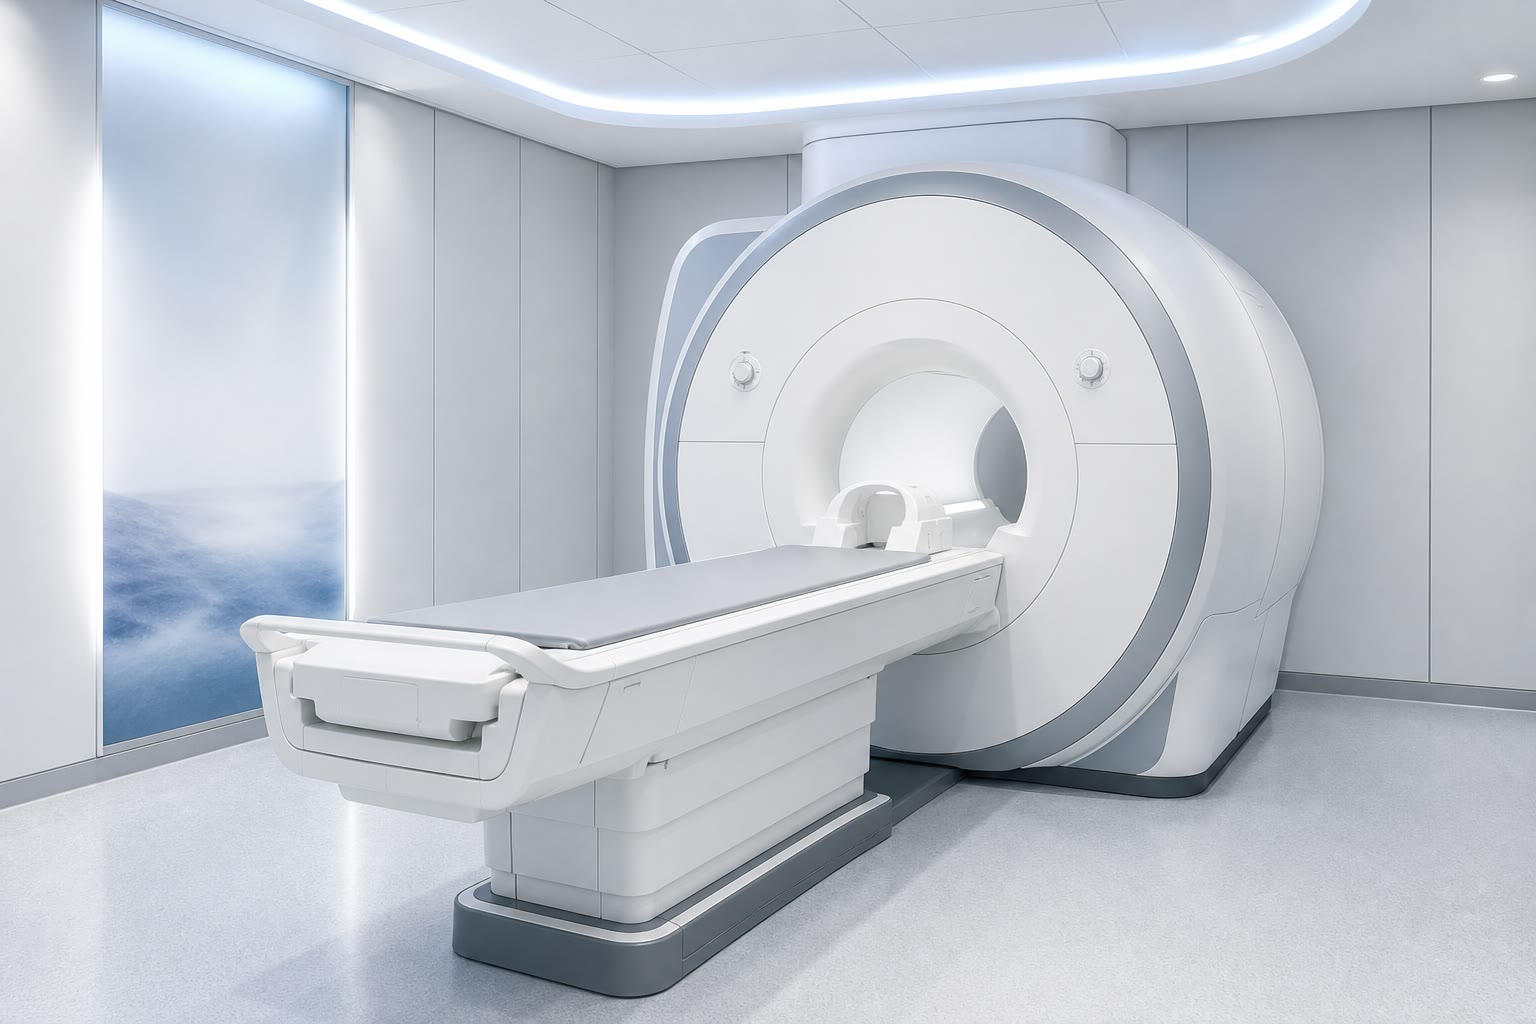
\includegraphics[width=0.58\linewidth]{images/book5/ai/b5-12-mri-scanner.jpg}

{\small MRI 扫描仪：超导磁场使人体质子\omterm{def:b3:spin-two-level:spin}{自旋}排列一致，射频脉冲使其偏转，其\omterm{prop:b3:spin-two-level:larmor}{拉莫尔进动}逐线圈读出——即本章的两能级物理，此处成像的是膝关节。}
\end{omfigure}

\section{练习}

\begin{exercise}[$\star$]\label{exo:b3:spin-two-level:1}
(a) 验证 $\sigma_x^2 = \sigma_y^2 = \sigma_z^2 = \mathbb 1$ 及
$\sigma_x\sigma_y = \iu\sigma_z$。(b) 推出 $[\hat S_x, \hat S_y]
= \iu\hbar\hat S_z$：二维情形下的角动量代数。
(c) 证明 $\hat S^2 = \tfrac34\hbar^2\,\mathbb 1$，并验证 $j(j+1)$
在 $j = \tfrac12$ 时的取值。(d) 证明任一 $2\times2$ 厄米矩阵都可写为
$\mathbb 1$ 与三个 $\sigma_i$ 的实系数线性组合。
\end{exercise}

\begin{exercise}[$\star$]\label{exo:b3:spin-two-level:2}
(a) 求 $\sigma_x$ 与 $\sigma_y$ 的归一化本征态。
(b) \omterm{def:b3:spin-two-level:spin}{自旋}制备在 $\ket{+x}$ 态，沿 $z$ 测量，结果
的概率为多少？(c) 沿 $y$ 测量呢？(d) 用布洛赫图像核验两者
（$\theta, \varphi$ 各为何值？）。
\end{exercise}

\begin{exercise}[$\star$]\label{exo:b3:spin-two-level:3}
三个串联的施特恩–格拉赫磁铁，轴依次为 $z$，然后是 $\vect n$，
它的倾角为 $\theta$，位于 $xz$ 平面内，再为 $z$；
每次均保留 $+$ 束。(a) 通过第二个磁铁的概率；(b)
通过全部三个磁铁的概率。(c) 取 $\theta = 90^\circ$，并
与\cref{ex:b3:spin-two-level:chained}比较。(d) 对于哪些
$\theta$ 值，三磁铁串联的通过概率最大，该结果
与\cref{exo:b3:quantum-formalism:5}中的内容有何呼应？
\end{exercise}

\begin{exercise}[$\star$]\label{exo:b3:spin-two-level:4}
计算能级分裂 $2|\mu|B$ 与共振频率，
在 \qty{1}{T} 磁场中，分别求 (a) 电子（$g = 2$）；(b)
质子（$\mu_p = 2.79\,\mu_{\text{N}}$，$\mu_{\text{N}} =
e\hbar/2m_{\text{p}}$）；(c) 将二者与 $k_{\text{B}}T$ 比较，温度为
\qty{300}{K}：电子与核\omterm{def:b3:spin-two-level:spin}{自旋}在
室温下的极化程度如何？(d) ESR 与 NMR 因此分别占据
光谱中的哪些波段？
\end{exercise}

\begin{exercise}[$\star\star$]\label{exo:b3:spin-two-level:5}
推导\omterm{prop:b3:spin-two-level:larmor}{拉莫尔进动}：取 $\hat H = -\gamma B_0\hat S_z$，(a)
计算 $\dd\langle\hat S_x\rangle/\dd t$，$\dd\langle\hat
S_y\rangle/\dd t$，$\dd\langle\hat S_z\rangle/\dd t$，由
\omterm{def:b3:quantum-formalism:commutator}{对易子}得出；(b) 求解 $\langle\hat{\vect S}\rangle(t)$，初始
\omterm{def:b3:spin-two-level:spin}{自旋}沿 $x$；(c) 证明 $\|\langle\hat{\vect S}\rangle\|$
及其与 $\vect B_0$ 的夹角均为常量；(d) 为何
\emph{能量本征态}图像（两个定态能级）与
\emph{进动}图像（一个转动的矢量）描述的是同一物理
——哪一个态在进动？
\end{exercise}

\begin{exercise}[$\star\star$]\label{exo:b3:spin-two-level:6}
(a) 验证 $\ket{+\vect n}$ 为
\cref{prop:b3:spin-two-level:bloch}中所断言的本征矢量。(b)
证明对映态相互正交。(c) 球面上，
$\sigma_x$ 与 $\sigma_y$ 的本征态分别位于何处？(d) 量子比特“非”门
将 $\ket\uparrow \leftrightarrow \ket\downarrow$ 互换，它对应球面的何种
旋转？又由
\cref{prop:b3:spin-two-level:rabi}中的哪种脉冲来实现它？
\end{exercise}

\begin{exercise}[$\star\star$]\label{exo:b3:spin-two-level:7}
旋转参考系，坦白说。取 $\hat H(t) = -\gamma(B_0\hat S_z
+ B_1[\hat S_x\cos\omega t - \hat S_y\sin\omega t])$：(a) 说明
为何转入以 $\omega$ 绕 $z$ 轴旋转的参考系，$B_0$ 被换为
$B_0 - \omega/\gamma$，$B_1$ 被冻结；(b) 共振时，
描述布洛赫矢量在旋转参考系中的运动；(c)
推导质子的 $\pi$ 脉冲时长，其中 $B_1 =
\qty{10}{\micro T}$；(d) 勾画实验室参考系中的观察者
在该脉冲期间所见的图像（两层嵌套的旋转）。
\end{exercise}

\begin{exercise}[$\star\star$]\label{exo:b3:spin-two-level:8}
21 cm 谱线。(a) 验证 $\Delta E = \qty{5.9}{\micro eV}$
给出 $\nu = \qty{1420}{MHz}$ 与 $\lambda = \qty{21.1}{cm}$。(b)
激发态的寿命为 $\qty{e7}{yr}$：其对应的谱线宽度为多少，
而观测到的宽度（$\sim$ kHz 及以上）为何完全是多普勒展宽？(c) 某星系
的盘缘以 \qty{220}{km/s} 相对其中心退行，
求其 21 cm 谱线轮廓的频率跨度。(d) 为何
21 cm 谱线示踪的是\emph{中性原子}气体，而 CO
（\cref{pb:b3:quantum-angular-momentum:1}）示踪的是\emph{分子}
气体——天文学家为何两者都需要？
\end{exercise}

\begin{exercise}[$\star\star$]\label{exo:b3:spin-two-level:9}
氨分子中的氮原子穿过 H$_3$ 平面发生隧穿：
两种“伞形”构型混合为对称态与反对称态，
二者能级劈裂 $\Delta E = \qty{e-4}{eV}$（
即本科二年级分册中的反转双重态）。(a) 论证
将氨分子视为两能级系统的合理性。(b) 跃迁频率与
波长。(c) 在微波激射器（1954 年）中，
经态选择的分子穿过谐振腔并放大该微波：入射束须满足
怎样的粒子数条件，它与热平衡情形有何不同？
(d) 在本科二年级分册所述光激光器问世前三年，
氨分子微波激射器演示了什么？
\end{exercise}

\begin{exercise}[$\star\star\star$]\label{exo:b3:spin-two-level:10}
\omterm{def:b3:spin-two-level:spin}{自旋}–轨道耦合，估算。在电子的静止参考系中，原子核
绕其运动：电子处于磁场 $B_{\text
{内}}$。(a) 由\cref{exo:b3:hydrogen-atom:10}(d)，取
$B_{\text{内}} \sim \qty{10}{T}$，对氢原子 $n = 2$ 估算
能级移动 $\mu_{\text{B}}B_{\text{内}}$，
并与\cref{exo:b3:hydrogen-atom:11}的精细结构标度比较。(b) 钠的
D 线在 \qty{589}{nm} 处劈裂 \qty{0.6}{nm}：换算为 meV
并换算为内场。(c) 为何劈裂随
$Z$ 急剧增大（内场大致按 $Z^4$ 与 $n^3$ 之比标度）？
(d) 各态以总角动量量子数 $j = l \pm \tfrac12$ 标记：数出
$p$ 能级的各态数，并检验没有遗漏。
\end{exercise}

\begin{exercise}[$\star\star\star$]\label{exo:b3:spin-two-level:11}
两\omterm{def:b3:spin-two-level:spin}{自旋}合成。对两个\omterm{def:b3:spin-two-level:spin}{自旋}为 $\tfrac12$ 的粒子，总
\omterm{def:b3:spin-two-level:spin}{自旋} $\hat{\vect S} = \hat{\vect S}_1 + \hat{\vect S}_2$。(a) 证明四个乘积态可重组为
\emph{三重态}（$S = 1$：
$\ket{\uparrow\uparrow}$，$(\ket{\uparrow\downarrow} +
\ket{\downarrow\uparrow})/\sqrt2$，$\ket{\downarrow\downarrow}$）
与\emph{单态}（$S = 0$：$(\ket{\uparrow\downarrow} -
\ket{\downarrow\uparrow})/\sqrt2$）——核对 $S_z$ 的计数，并
对中间两态考察 $\hat S^2$ 的作用（取 $\hat
S^2 = \hat S_1^2 + \hat S_2^2 + 2\hat{\vect S}_1\cdot\hat{\vect
S}_2$ 与 $\hat{\vect S}_1\cdot\hat{\vect S}_2 = \tfrac12(\hat
S_{1+}\hat S_{2-} + \hat S_{1-}\hat S_{2+}) + \hat S_{1z}\hat
S_{2z}$）。(b) 四个态中哪一个是纠缠态，即无法写成
乘积形式？(c) 氢原子的超精细能级对
（\cref{ex:b3:spin-two-level:hyperfine}）恰好就是这里的三重态与
单态：已知该谱线
在 21 cm 处\emph{发射}，哪个能级更高？(d) 单态的两\omterm{def:b3:spin-two-level:spin}{自旋}
在\emph{每一}方向上完全反关联：沿任一方向
$\vect n$ 测量其中之一，另一个给出相反结果。为何这种
关联无论多么醒目，都不能传递任何信号？
\end{exercise}

\begin{exercise}[$\star\star\star$]\label{exo:b3:spin-two-level:12}
定义秒的钟。铯的基态超精细劈裂恰为
$\qty{9192631770}{Hz}$（由秒的定义给出）。在喷泉钟中，
原子先接受一个 $\pi/2$ 脉冲，再自由飞行
$T = \qty{0.5}{s}$，随后接受第二个 $\pi/2$ 脉冲；转移的
分数按 $\cos^2(\pi\,\delta\,T)$ 随失谐 $\delta$ 振荡
（拉姆齐条纹——接受此结论即可）。(a) 用
布洛赫语言说明每个 $\pi/2$ 脉冲与自由飞行的作用。(b)
中央条纹的宽度。(c) 若信噪比允许将
条纹中心可分辨到 $10^4$ 分之一，
则所得频率的相对精度为多少？(d) 为何光学钟（皮赫兹跃迁）
在相同的条纹分辨能力下胜过微波钟——以
约多少倍计？
\end{exercise}

\section{问题：观察人体内部}

\begin{problem}[{周末问题——磁共振成像，
从自旋到扫描}]\label{pb:b3:spin-two-level:1}
人体约三分之二是水；每个水分子含两个
质子，每个质子都是一个\omterm{def:b3:spin-two-level:spin}{自旋}为 $\tfrac12$ 的小磁铁。将人置于强
磁场中，以质子的拉莫尔频率轻轻激发它们，然后聆听：
这就是\omterm{prop:b3:spin-two-level:rabi}{磁共振}成像，即将\omterm{def:b3:spin-two-level:spin}{自旋}物理用于医学。数据：
$\gamma_{\text{p}}/2\pi = \qty{42.58}{MHz/T}$；$B_0 = \qty{3.0}{T}$；
组织中的质子数密度 $n \approx \qty{6.6e28}{m^{-3}}$；
\qty{310}{K} 时 $k_{\text{B}}T$ 为 \qty{26.7}{meV}；$h =
\qty{4.14e-15}{eV.s}$。

\medskip\noindent\textbf{第一部分——磁铁中的\omterm{def:b3:spin-two-level:spin}{自旋}。}
\begin{enumerate}
  \item 计算 \qty{3.0}{T} 下的拉莫尔频率，以及光子
        能量 $h\nu$（以 eV 为单位）。
  \item 计算两个质子
        能级之间的粒子数不平衡 $\Delta n/n \approx h\nu/2k_{\text{B}}T$。
  \item 只有这部分超额——百万分之几——贡献信号：
        每立方厘米组织中有多少个“有用”
        质子？
  \item 为何此处的热极化如此微弱，而
        斯特恩–格拉赫束已被完全分裂？（两种实验各测量什么：
        单原子\omterm{def:b3:quantum-formalism:observable}{本征值}，还是热
        平均？）
  \item 将 $B_0$ 加倍，对信号有何影响（两种效应：极化与
        更高频率下的感应电动势）？为何医院愿为
        更大的磁铁付费？
  \item 磁铁为超导且始终开启：为何
        房间里一个松动的钢制氧气瓶会成为致命的抛体
        （\cref{ex:b3:spin-two-level:stern-gerlach}中的哪一种力
        作用于它？）
\end{enumerate}

\medskip\noindent\textbf{第二部分——脉冲与回波。}
\begin{enumerate}[resume]
  \item 一个横向线圈在共振条件下施加 $B_1 = \qty{10}{\micro T}$，
        计算拉比频率，以及
        $\pi/2$ 脉冲和 $\pi$ 脉冲的时长。
  \item 施加 $\pi/2$ 脉冲之后，磁化强度如何变化，
        法拉第电磁感应定律在接收线圈中感应出什么
        （在何种频率下）？
  \item 横向信号以时间常数 $T_2$ 衰减
        （\omterm{def:b3:spin-two-level:spin}{自旋}在彼此的场及局域
        非均匀性中失相）；纵向磁化
        以 $T_1$ 重新增长（能量流入组织）。典型值为：
        $T_1 \approx \qty{1}{s}$，$T_2 \approx \qty{0.1}{s}$。为何
        相干时间永远不可能远超能量弛豫时间（
        每一次与能量交换的翻转会
        如何改变相位？）
  \item \omterm{def:b3:spin-two-level:spin}{自旋}回波：施加 $\pi/2$ 脉冲并经过时延 $\tau$ 后，
        再施加 $\pi$ 脉冲，在 $2\tau$ 时刻，失相的
        \omterm{def:b3:spin-two-level:spin}{自旋}重新对齐，信号复现。请解释这一技巧，
        并以在跑道上被要求掉头的跑者为例。
  \item 回波能抵消哪一种衰减——是来自
        \emph{静态}场非均匀性引起的失相，还是来自
        涨落的分子场所致的失相——为何只抵消这一种？
  \item 不同组织的 $T_1$、$T_2$ 各不相同（脂肪：
        $T_1$ 短；水／液体：长；许多肿瘤：$T_2$
        长于宿主组织）。一句话概括：脉冲序列的时序如何
        把弛豫时间转化为图像
        \emph{对比度}？
\end{enumerate}

\medskip\noindent\textbf{第三部分——从信号到图像。}
\begin{enumerate}[resume]
  \item 叠加梯度 $G = \qty{40}{mT/m}$，沿 $z$ 方向：
        拉莫尔频率随位置变化。计算
        $\dd\nu/\dd z$，单位为千赫每毫米。
  \item 一个仅包含频带 $\nu_0 \pm
        \qty{1}{kHz}$ 的整形射频脉冲激发人体的哪一层？（
        层面选择。）
  \item 读出期间，沿 $x$ 方向的梯度使层面中的每一列
        各自发出自己的频率：哪种数学运算
        可将接收到的时间信号转换为空间分布
        （回想本科二年级分册中的傅里叶工具）？
  \item 估算扫描的总信息量：一幅 $256 \times 256$
        的图像（12 位），以及为何逐行采集
        （每行一个回波，重复时间 $\sim T_1$）使
        一次扫描耗时数分钟。
  \item 患者听到剧烈的敲击声：是什么在机械地
        撞击（想想梯度线圈在
        \qty{3}{T} 磁场中切换时，是哪一种力？）
  \item X 射线成像对比的是电子密度；\omterm{prop:b3:spin-two-level:rabi}{磁共振}成像对比的是
        质子密度\emph{和}弛豫：为何\omterm{prop:b3:spin-two-level:rabi}{磁共振}是
        软组织与大脑的首选工具，它给出的电离
        辐射剂量是多少？
\end{enumerate}

\medskip\noindent\textbf{第四部分——\omterm{def:b3:spin-two-level:spin}{自旋}的其他用途。}
\begin{enumerate}[resume]
  \item 化学家以 \qty{10}{ppm} 的分辨率做同样的实验：
        电子云会轻微屏蔽每个原子核，使其共振
        频率发生移动（即“化学位移”）。为何
        这一现象使核\omterm{prop:b3:spin-two-level:rabi}{磁共振}成为分子的“指纹”？
  \item 功能\omterm{prop:b3:spin-two-level:rabi}{磁共振}成像可描绘思维活动：脱氧血红蛋白
        具有顺磁性，并缩短局域的 $T_2^*$。请追踪
        从神经活动到图像亮度的完整链条。
  \item 用\emph{电子}的磁矩做同样的拉莫尔物理，
        运行频率为 \qty{84}{GHz}，磁场为 \qty{3}{T}：为何电子
        共振在人体内毫无用处，却在研究自由基和缺陷时
        极为珍贵？
  \item 将第 1 项中光子的能量与典型的
        化学键能相比较，说明“非电离”一词的理由，并与
        \qty{60}{keV} 的 X 射线光子作对比。
  \item 十 ppm 的极化可以被增强：激光极化的
        氙气可达到数量级为一的极化，被吸入以
        成像肺部气腔。每个原子核的信号大致
        提高多少倍，而气体的低密度为何
        仍使此技巧必不可少？
  \item 硅类晶体管式势阱中的单个电子\omterm{def:b3:spin-two-level:spin}{自旋}
        现已可用正是本章的这些脉冲，将其作为量子比特读出和驱动：
        请说出两项使其值得推荐的\omterm{def:b3:spin-two-level:spin}{自旋}性质（
        \omterm{def:b3:quantum-formalism:state}{希尔伯特空间}的大小；与噪声耦合的微弱程度
        ）。
  \item 概括这一著名结果：一个 \qty{128}{MHz} 的\omterm{def:b3:spin-two-level:spin}{自旋}进动、
        百万分之十的热极化、
        两只弛豫“时钟”与三个磁场梯度便足以
        对活体大脑做分层成像——斯特恩和格拉赫的
        两个斑点，发展成了一座医院。
\end{enumerate}
\end{problem}
